\documentclass[tikz, border=15pt]{standalone}
\usepackage{amsmath}
\usetikzlibrary{calc, patterns}

% Define the exact colors from your prompt
\definecolor{mygreen}{HTML}{00d1b2}
\definecolor{myred}{HTML}{ff6b6b}
\definecolor{myblue}{HTML}{4facfe}

\begin{document}
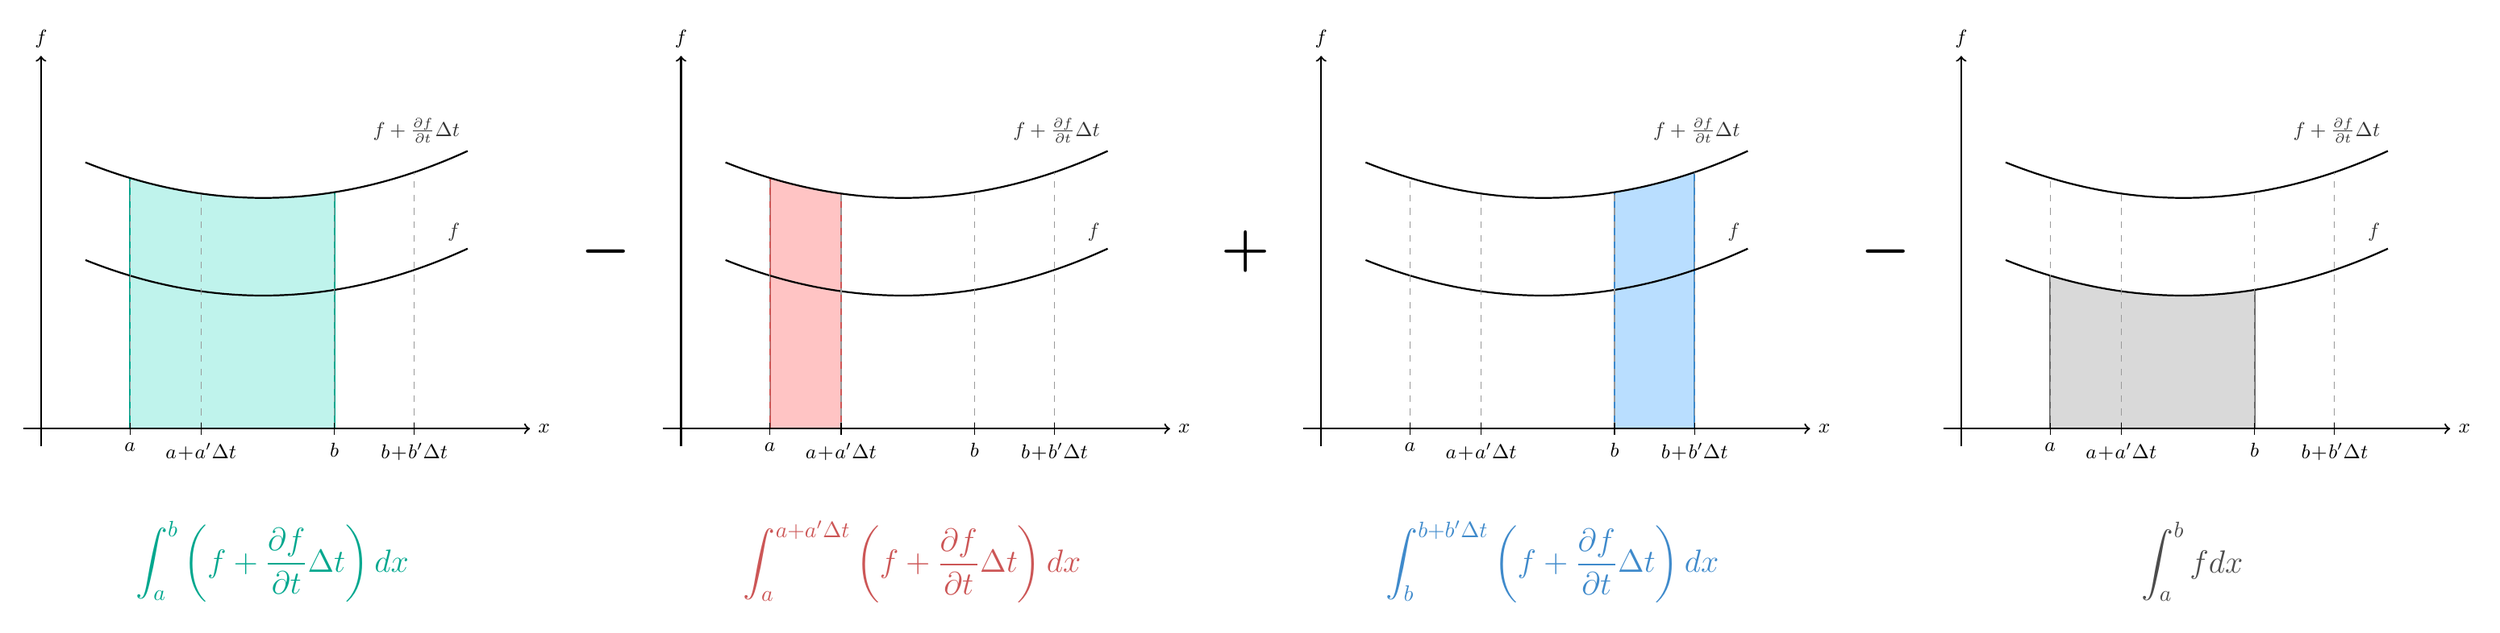
\begin{tikzpicture}[
    scale=1.4, % Adjusted scale for 1x4 layout
    every node/.style={font=\small},
    label box/.style={align=center}
]

    % --- 1. DEFINE SHARED FUNCTIONS AND VARIABLES ---
    % Bottom curve: f(t, x)
    \pgfmathdeclarefunction{funcF}{1}{\pgfmathparse{0.1*(#1-2.5)^2 + 1.5}}
    % Top curve: f(t, x) + df/dt * dt
    \pgfmathdeclarefunction{funcFdt}{1}{\pgfmathparse{0.1*(#1-2.5)^2 + 2.6}}

    \def\a{1.0} 
    \def\da{0.8} 
    \pgfmathsetmacro{\anew}{\a + \da}
    
    \def\b{3.3} 
    \def\db{0.9} 
    \pgfmathsetmacro{\bnew}{\b + \db}

    % \W is the horizontal step between each sub-diagram
    \def\W{7.2} 

    % --- 2. MACRO TO DRAW THE BASE SCENE EVERY TIME ---
    \def\drawBase{
        % Axes
        \draw[->, thick] (-0.2,0) -- (5.5,0) node[right] {$x$};
        \draw[->, thick] (0,-0.2) -- (0,4.2) node[above] {$f$};

        % Curves
        \draw[thick] plot[domain=0.5:4.8, samples=100] (\x, {funcF(\x)});
        \draw[thick] plot[domain=0.5:4.8, samples=100] (\x, {funcFdt(\x)});

        % Curve Labels
        \node[above left, text=black!80] at (4.8, {funcF(4.8)}) {$f$};
        \node[above left, text=black!80] at (4.8, {funcFdt(4.8)}) {$f + \frac{\partial f}{\partial t}\Delta t$};

        % Dashed Boundary Lines
        \draw[dashed, thin, gray!80] (\a,0) -- (\a, {funcFdt(\a)});
        \draw[dashed, thin, gray!80] (\b,0) -- (\b, {funcFdt(\b)});
        \draw[dashed, thin, gray!80] (\anew,0) -- (\anew, {funcFdt(\anew)});
        \draw[dashed, thin, gray!80] (\bnew,0) -- (\bnew, {funcFdt(\bnew)});

        % X-Axis Marks
        \draw (\a, 2pt) -- (\a, -2pt) node[below] {$a$};
        \draw (\b, 2pt) -- (\b, -2pt) node[below] {$b$};
        \draw (\anew, 2pt) -- (\anew, -2pt) node[below] {$a \!+\! a'\Delta t$};
        \draw (\bnew, 2pt) -- (\bnew, -2pt) node[below] {$b \!+\! b'\Delta t$};
    }


    % ==========================================
    % PANEL 1: (The Green Area)
    % ==========================================
    \begin{scope}[shift={(0,0)}]
        % Fill Area
        \fill[mygreen, fill opacity=0.25] (\a,0) -- plot[domain=\a:\b, samples=100] (\x, {funcFdt(\x)}) -- (\b,0) -- cycle;
        \draw[mygreen!80!black, thick] (\a,0) -- (\a, {funcFdt(\a)});
        \draw[mygreen!80!black, thick] (\b,0) -- (\b, {funcFdt(\b)});
        
        \drawBase % Overlay base scene
        
        % Label below
        \node[label box, text=mygreen!80!black] at (2.6, -1.5) 
            {\Large $\displaystyle \int_a^b \left(f + \frac{\partial f}{\partial t}\Delta t\right) dx$};
    \end{scope}

    % Operator -
    \node at (1*\W - 0.85, 2.0) {\Huge $\boldsymbol{-}$};

    % ==========================================
    % PANEL 2: (The Red Area)
    % ==========================================
    \begin{scope}[shift={(1*\W,0)}]
        % Fill Area
        \fill[myred, fill opacity=0.4] (\a,0) -- plot[domain=\a:\anew, samples=50] (\x, {funcFdt(\x)}) -- (\anew,0) -- cycle;
        \draw[myred!80!black, thick] (\a,0) -- (\a, {funcFdt(\a)});
        \draw[myred!80!black, thick] (\anew,0) -- (\anew, {funcFdt(\anew)});
        
        \drawBase % Overlay base scene
        
        % Label below
        \node[label box, text=myred!80!black] at (2.6, -1.5) 
            {\Large $\displaystyle \int_a^{a + a'\Delta t} \left(f + \frac{\partial f}{\partial t}\Delta t\right) dx$};
    \end{scope}

    % Operator +
    \node at (2*\W - 0.85, 2.0) {\Huge $\boldsymbol{+}$};

    % ==========================================
    % PANEL 3: (The Blue Area)
    % ==========================================
    \begin{scope}[shift={(2*\W,0)}]
        % Fill Area
        \fill[myblue, fill opacity=0.4] (\b,0) -- plot[domain=\b:\bnew, samples=50] (\x, {funcFdt(\x)}) -- (\bnew,0) -- cycle;
        \draw[myblue!80!black, thick] (\b,0) -- (\b, {funcFdt(\b)});
        \draw[myblue!80!black, thick] (\bnew,0) -- (\bnew, {funcFdt(\bnew)});
        
        \drawBase % Overlay base scene
        
        % Label below
        \node[label box, text=myblue!80!black] at (2.6, -1.5) 
            {\Large $\displaystyle \int_b^{b + b'\Delta t} \left(f + \frac{\partial f}{\partial t}\Delta t\right) dx$};
    \end{scope}

    % Operator -
    \node at (3*\W - 0.85, 2.0) {\Huge $\boldsymbol{-}$};

    % ==========================================
    % PANEL 4: (The Gray Area)
    % ==========================================
    \begin{scope}[shift={(3*\W,0)}]
        % Fill Area
        \fill[black, fill opacity=0.15] (\a,0) -- plot[domain=\a:\b, samples=100] (\x, {funcF(\x)}) -- (\b,0) -- cycle;
        \draw[black!60, thick] (\a,0) -- (\a, {funcF(\a)});
        \draw[black!60, thick] (\b,0) -- (\b, {funcF(\b)});
        
        \drawBase % Overlay base scene
        
        % Label below
        \node[label box, text=black!70] at (2.6, -1.5) 
            {\Large $\displaystyle \int_a^b f dx$};
    \end{scope}

\end{tikzpicture}
\end{document}